% Standalone TikZ figure: MobileNetV4-small multi-view retrieval encoder with FULL-RANK
% fine-cell heads and strong augmentation (T6/R9, fold-0 126.04km, 2026-08-30).
%
% This is the BEST result of the geo-cell classification line -- it supersedes T6/E3e
% (architecture_t6_e3e.tex, 137.16km) and is the model referred to in the git history as
% "Until 126.0km median reached". It is still NOT the project's best overall result: the
% convnextv2_femto pure-retrieval model reaches 59.22km pooled OOF (best_result/README.md)
% and is a different architecture class (no cells, no country head, no offset head).
%
% Kept as a separate file per this project's convention of not overwriting earlier
% architecture figures (see architecture_t3_4.tex / architecture_t4_1c.tex header notes).
% Deltas from architecture_t6_e3e.tex are marked NEW.
%
% Compile alone:      tectonic architecture_t6_r9.tex   (or pdflatex/lualatex/xelatex)
%
% Every value below is read from the run's own artefacts, not from the working notes:
%   failed_experiments/_superseded_T2_to_T6/T6_R9_mnv4_strongaug_fold0/
%     config.json, param_compliance.json, fold0/fold_result.json, fold0/history.json
%   Parameter breakdown verified by reading tensor shapes directly out of
%   fold0/best_model.pt (see the note at the end of this file).
%
% THE CENTRAL IDEA -- a parameter rebalance, not a better network:
%   E3e spent 81% of the 5M budget on the backbone and squeezed the cell heads through a
%   low-rank trunk to make them fit. R9 does the opposite: a SMALLER backbone
%   (mobilenetv4_conv_small, 2.49M vs EfficientNet-B0's 4.01M) frees 1.51M params, which
%   are spent on FULL-RANK direct cell heads (1.89M, 40% of the whole budget).
%   The bottleneck was classification capacity, so buying capacity with backbone strength
%   was the winning trade -- 137.16km -> 126.04km.
%   This was idea "E. Smaller backbone to buy classification capacity" in T6_FINDINGS.md,
%   filed there as *speculative, low priority*. It produced the largest single-model gain
%   of the entire cell line.

\documentclass[tikz,border=4pt]{standalone}
\usepackage{amsmath}
\usetikzlibrary{positioning, arrows.meta, fit, backgrounds, shapes.geometric, calc}

\begin{document}
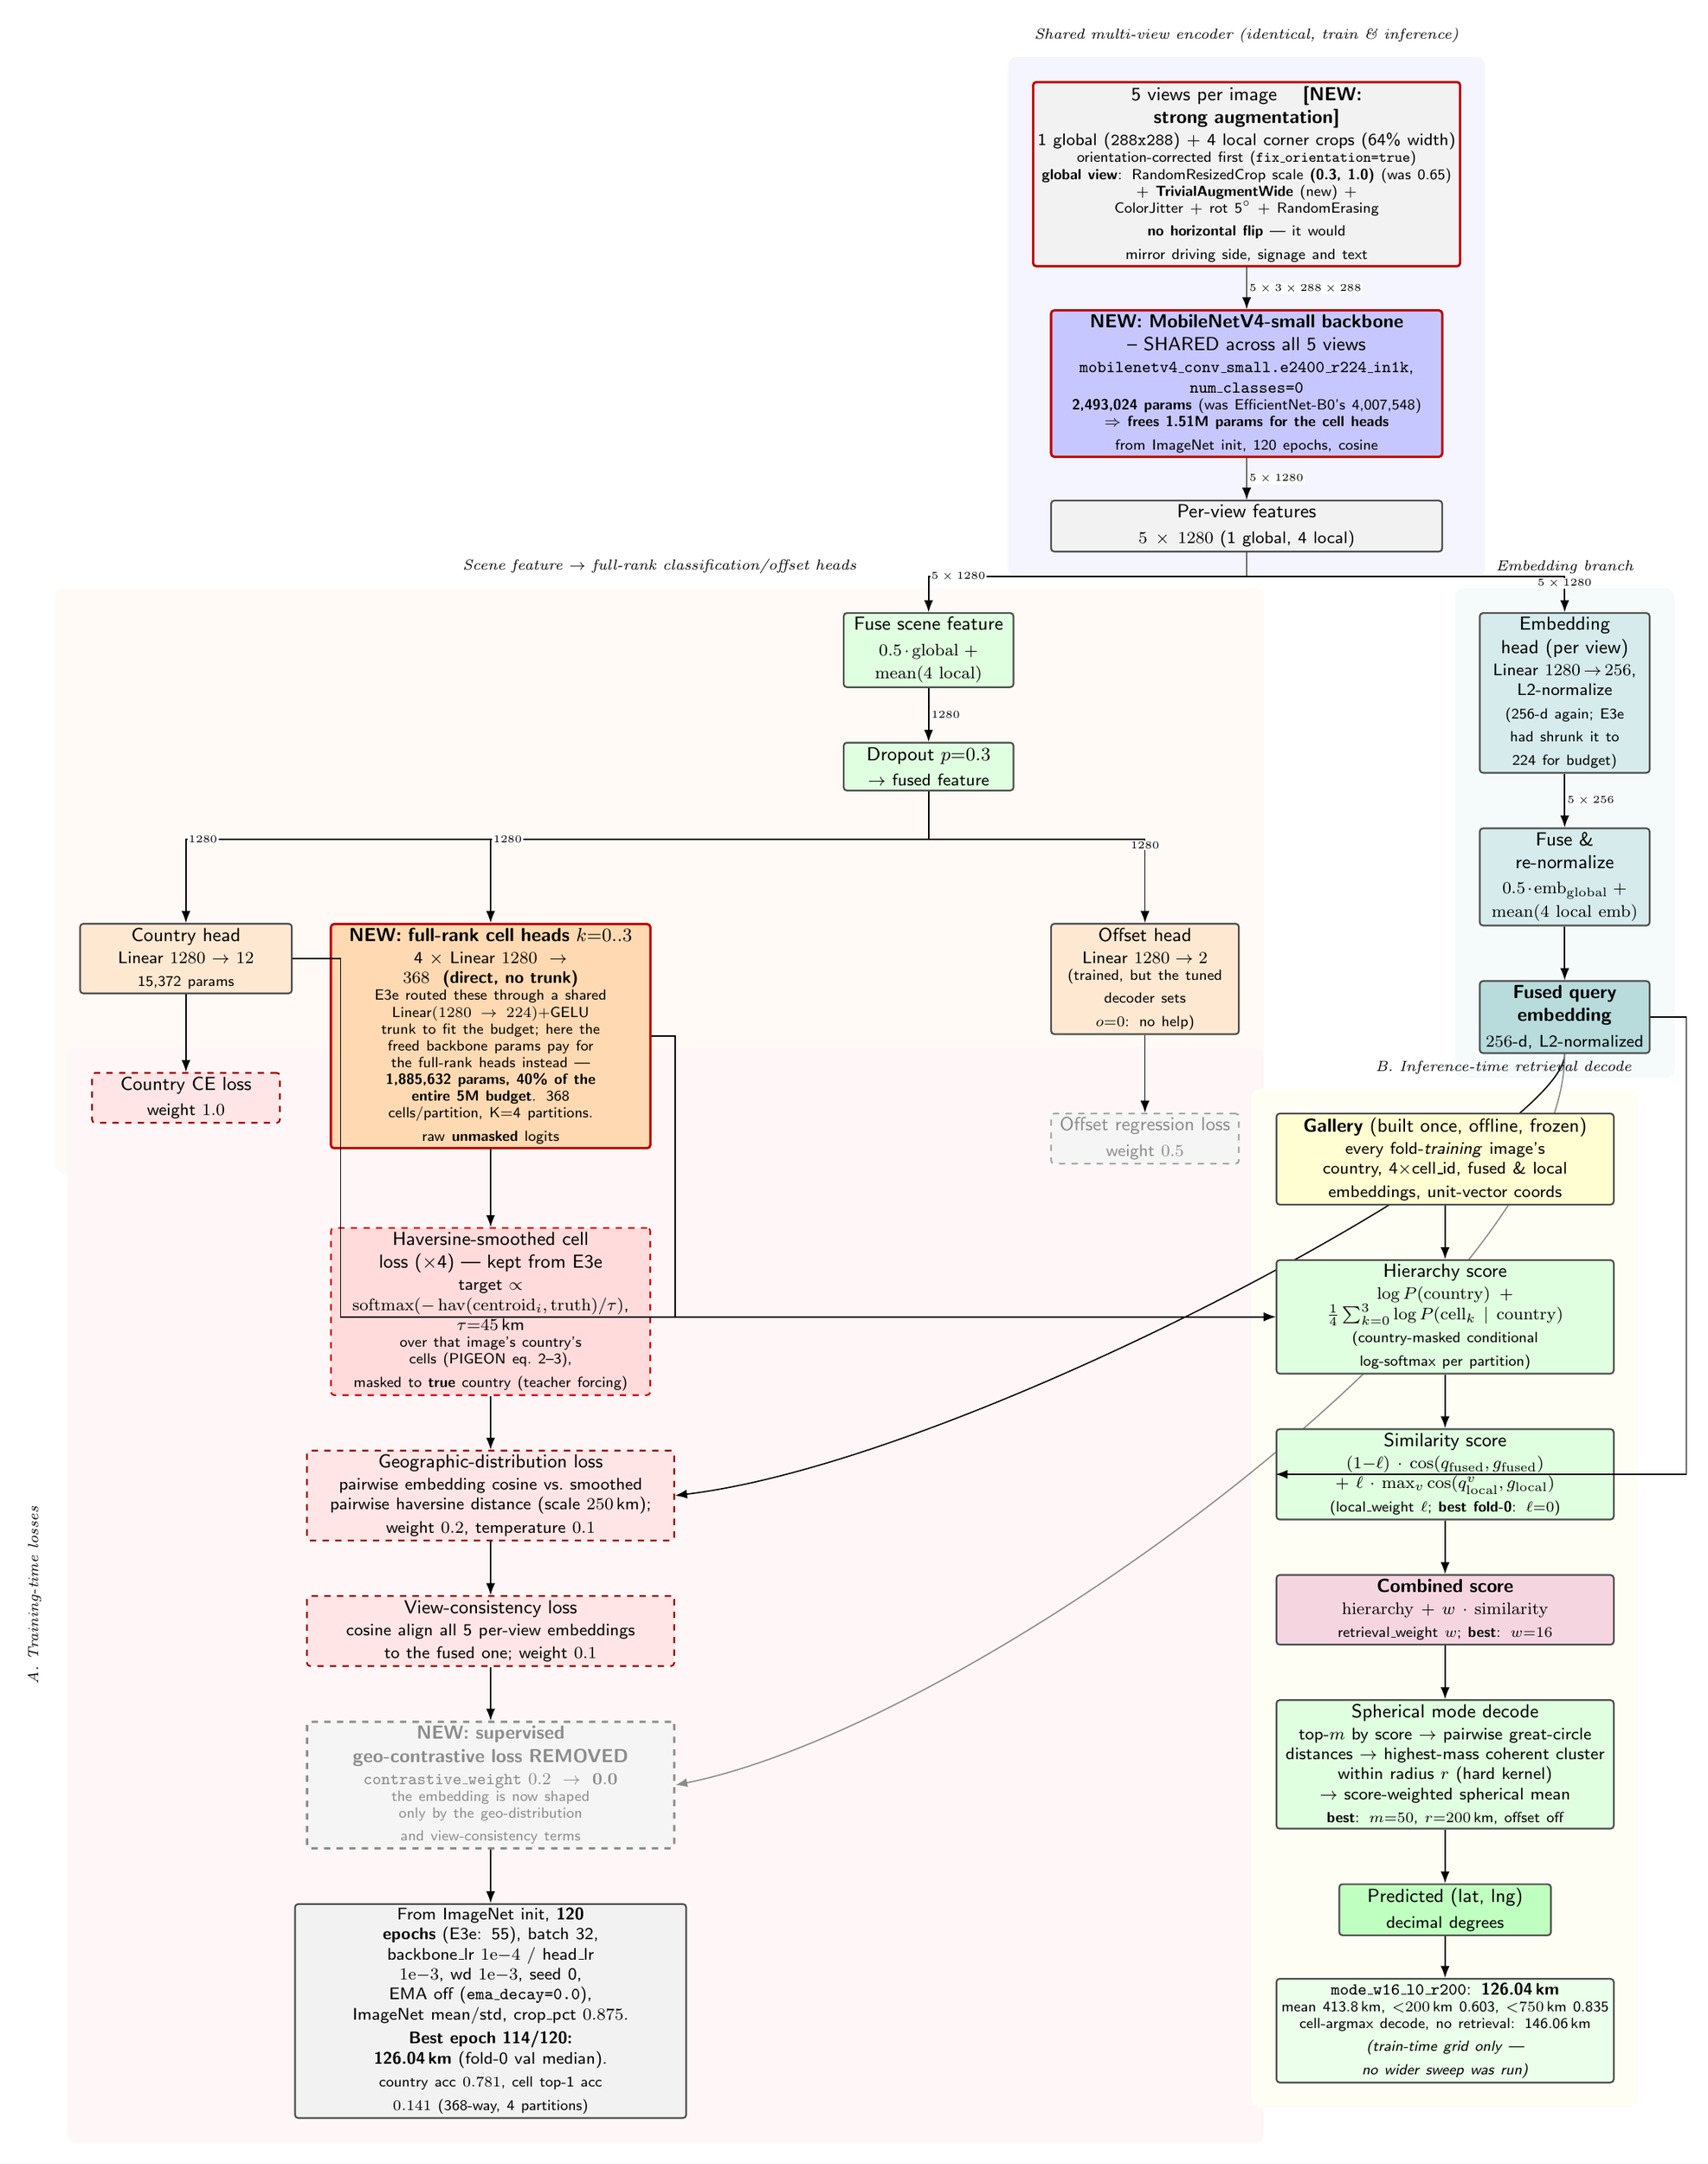
\begin{tikzpicture}[
  font=\sffamily\small,
  execute at begin picture={\hyphenpenalty=10000\exhyphenpenalty=10000\relax},
  node distance=7mm and 9mm,
  >={Latex[length=2mm,width=1.5mm]},
  every path/.style={line width=0.6pt},
  block/.style={
    rectangle, rounded corners=1.5pt, draw=black!70, thick,
    minimum height=8mm, text width=30mm, align=center, inner sep=2pt
  },
  backbone/.style={block, fill=blue!12, text width=64mm},
  head/.style={block, fill=orange!18, text width=27mm},
  emb/.style={block, fill=teal!16, text width=27mm},
  op/.style={block, fill=green!12, text width=27mm},
  fuse/.style={block, fill=purple!16, thick, text width=40mm},
  loss/.style={block, fill=red!10, dashed, draw=red!60!black, text width=30mm},
  offloss/.style={block, fill=black!4, dashed, draw=black!35, text=black!45, text width=30mm},
  gallery/.style={block, fill=yellow!18, text width=32mm},
  outnode/.style={block, fill=green!25, thick, text width=34mm},
  newbox/.style={draw=red!75!black, line width=1.1pt},
  dimlabel/.style={font=\tiny\itshape, pos=0.5, right=0.5pt, fill=white, inner sep=0.5pt},
  dimlabelb/.style={font=\tiny\itshape, pos=0.5, below=0.5pt, fill=white, inner sep=0.5pt},
]

% =========================================================================================
% SHARED ENCODER
% =========================================================================================
\node[block, fill=black!5, text width=70mm, newbox] (input)
  {5 views per image \quad \textbf{[NEW: strong augmentation]}\\[1pt]
   \footnotesize 1 global (\texttt{288x288}) $+$ 4 local corner crops (64\% width)\\
   \scriptsize orientation-corrected first (\texttt{fix\_orientation=true})\\
   \textbf{global view}: RandomResizedCrop scale \textbf{(0.3, 1.0)} (was 0.65)\\
   $+$ \textbf{TrivialAugmentWide} (new) $+$ ColorJitter $+$ rot 5$^\circ$ $+$ RandomErasing\\
   \textbf{no horizontal flip} --- it would mirror driving side, signage and text};
\node[backbone, below=of input, newbox, fill=blue!22] (backbone)
  {\textbf{NEW: MobileNetV4-small backbone} -- SHARED across all 5 views\\[1pt]
   \footnotesize\texttt{mobilenetv4\_conv\_small.e2400\_r224\_in1k}, \texttt{num\_classes=0}\\
   \scriptsize \textbf{2,493,024 params} (was EfficientNet-B0's 4,007,548)\\
   $\Rightarrow$ \textbf{frees 1.51M params for the cell heads}\\
   from ImageNet init, 120 epochs, cosine};
\draw[->] (input) -- (backbone) node[dimlabel]{$5\times3\times288\times288$};

\node[block, fill=black!5, below=of backbone, text width=64mm] (perview)
  {Per-view features\\[1pt]\footnotesize $5 \times 1280$ (1 global, 4 local)};
\draw[->] (backbone) -- (perview) node[dimlabel]{$5\times1280$};

% ---- split: scene-feature path (left) vs. embedding path (right) ----
\node[op, below left=10mm and 6mm of perview] (fuse_feat)
  {Fuse scene feature\\[1pt]\footnotesize $0.5\!\cdot\!\mathrm{global} + \mathrm{mean}(4\ \mathrm{local})$};
\node[emb, below right=10mm and 6mm of perview] (emb_head)
  {Embedding head (per view)\\[1pt]\footnotesize Linear $1280\!\to\!256$, L2-normalize\\
   \scriptsize (256-d again; E3e had shrunk it to 224 for budget)};

\draw[->] (perview.south) -- ++(0,-4mm) -| (fuse_feat.north) node[pos=0.3,dimlabel]{$5\times1280$};
\draw[->] (perview.south) -- ++(0,-4mm) -| (emb_head.north) node[pos=0.7,dimlabelb]{$5\times1280$};

\node[op, below=9mm of fuse_feat] (dropout)
  {Dropout $p{=}0.3$\\[1pt]\footnotesize $\to$ fused feature};
\draw[->] (fuse_feat) -- (dropout) node[dimlabel]{$1280$};

\node[emb, below=9mm of emb_head] (fuse_emb)
  {Fuse \& re-normalize\\[1pt]\footnotesize $0.5\!\cdot\!\mathrm{emb}_{\mathrm{global}} + \mathrm{mean}(4\ \mathrm{local\ emb})$};
\draw[->] (emb_head) -- (fuse_emb) node[dimlabel]{$5\times256$};

\node[emb, below=9mm of fuse_emb, fill=teal!28, thick] (final_emb)
  {\textbf{Fused query embedding}\\[1pt]\footnotesize $256$-d, L2-normalized};
\draw[->] (fuse_emb) -- (final_emb);

% ---- heads: country, DIRECT full-rank K=4 cell heads (no trunk), offset ----
\node[head, below left=22mm and 92mm of dropout, text width=34mm] (country_head)
  {Country head\\[1pt]\footnotesize Linear $1280\!\to\!12$\\ \scriptsize 15,372 params};
\node[head, below left=22mm and 32mm of dropout, newbox, fill=orange!30, text width=52mm] (cell_heads)
  {\textbf{NEW: full-rank cell heads} $k{=}0..3$\\[1pt]
   \footnotesize 4 $\times$ Linear $1280\!\to\!368$ \ \textbf{(direct, no trunk)}\\
   \scriptsize E3e routed these through a shared Linear$(1280\!\to\!224)$+GELU\\
   trunk to fit the budget; here the freed backbone params pay for\\
   the full-rank heads instead --- \textbf{1,885,632 params, 40\% of the\\
   entire 5M budget}. 368 cells/partition, K$=$4 partitions.\\
   raw \textbf{unmasked} logits};
\node[head, below right=22mm and 6mm of dropout, text width=30mm] (offset_head)
  {Offset head\\[1pt]\footnotesize Linear $1280\!\to\!2$\\
   \scriptsize (trained, but the tuned\\ decoder sets $o{=}0$: no help)};

\draw[->] (dropout.south) -- ++(0,-8mm) -| (country_head.north) node[pos=0.25,dimlabel]{$1280$};
\draw[->] (dropout.south) -- ++(0,-8mm) -| (cell_heads.north) node[pos=0.4,dimlabel]{$1280$};
\draw[->] (dropout.south) -- ++(0,-8mm) -| (offset_head.north) node[pos=0.75,dimlabelb]{$1280$};

% =========================================================================================
% A. TRAINING-TIME LOSSES
% =========================================================================================
\node[loss, below=13mm of country_head] (l_country)
  {Country CE loss\\[1pt]\footnotesize weight $1.0$};
\draw[->] (country_head) -- (l_country);

\node[loss, below=13mm of cell_heads, draw=red!85!black, fill=red!14, text width=52mm] (l_cell)
  {Haversine-smoothed cell loss ($\times$4) --- kept from E3e\\[1pt]
   \footnotesize target $\propto\ \mathrm{softmax}\!\left(-\,\mathrm{hav}(\mathrm{centroid}_i, \mathrm{truth})/\tau\right)$,
   $\tau{=}45$\,km\\
   \scriptsize over that image's country's cells (PIGEON eq.~2--3),\\
   masked to \textbf{true} country (teacher forcing)};
\draw[->] (cell_heads) -- (l_cell);

\node[offloss, below=13mm of offset_head] (l_offset)
  {Offset regression loss\\[1pt]\footnotesize weight $0.5$};
\draw[->] (offset_head) -- (l_offset);

\node[loss, below=9mm of l_cell, text width=60mm] (l_geo)
  {Geographic-distribution loss\\[1pt]\footnotesize pairwise embedding cosine vs.\ smoothed\\
   pairwise haversine distance (scale $250$\,km);\\ weight $0.2$, temperature $0.1$};
\draw[->] (final_emb.south) .. controls +(0,-14mm) and +(50mm,6mm) .. (l_geo.east);
\draw[->] (l_cell) -- (l_geo);

\node[loss, below=9mm of l_geo, text width=60mm] (l_consist)
  {View-consistency loss\\[1pt]\footnotesize cosine align all 5 per-view embeddings\\
   to the fused one; weight $0.1$};
\draw[->] (l_geo) -- (l_consist);

\node[offloss, below=9mm of l_consist, text width=60mm, newbox, draw=black!45] (l_contrastive)
  {\textbf{NEW: supervised geo-contrastive loss REMOVED}\\[1pt]
   \footnotesize \texttt{contrastive\_weight} $0.2 \to \mathbf{0.0}$\\
   \scriptsize the embedding is now shaped only by the geo-distribution\\
   and view-consistency terms};
\draw[->] (l_consist) -- (l_contrastive);
\draw[->,black!45] (final_emb.south) .. controls +(0,-40mm) and +(50mm,10mm) .. (l_contrastive.east);

\node[block, fill=black!5, below=9mm of l_contrastive, text width=64mm] (trainnote)
  {\footnotesize From ImageNet init, \textbf{120 epochs} (E3e: 55), batch 32,\\
   backbone\_lr $1\mathrm{e}{-4}$ / head\_lr $1\mathrm{e}{-3}$, wd $1\mathrm{e}{-3}$, seed 0,\\
   EMA off (\texttt{ema\_decay=0.0}), ImageNet mean/std, crop\_pct $0.875$.\\[2pt]
   \textbf{Best epoch 114/120: 126.04\,km} (fold-0 val median).\\
   \scriptsize country acc $0.781$, cell top-1 acc $0.141$ (368-way, 4 partitions)};
\draw[->] (l_contrastive) -- (trainnote);

% =========================================================================================
% B. INFERENCE-TIME RETRIEVAL DECODE (unchanged from E3e)
% =========================================================================================
\node[gallery, below right=13mm and 6mm of offset_head, text width=55mm] (gallery_build)
  {\textbf{Gallery} (built once, offline, frozen)\\[1pt]\footnotesize every fold-\emph{training} image's\\
   country, 4$\times$cell\_id, fused \& local\\ embeddings, unit-vector coords};

\node[op, below=9mm of gallery_build, text width=55mm] (hierarchy_score)
  {Hierarchy score\\[1pt]\footnotesize $\log P(\mathrm{country}) + \tfrac{1}{4}\sum_{k=0}^{3}\log P(\mathrm{cell}_k\!\mid\!\mathrm{country})$\\
   \scriptsize (country-masked conditional log-softmax per partition)};
\draw[->] (country_head.east) -- ++(8mm,0) |- (hierarchy_score.west);
\draw[->] (cell_heads.east) -- ++(4mm,0) |- (hierarchy_score.west);
\draw[->] (gallery_build) -- (hierarchy_score);

\node[op, below=9mm of hierarchy_score, text width=55mm] (sim_score)
  {Similarity score\\[1pt]\footnotesize $(1{-}\ell)\cdot\cos(q_{\mathrm{fused}}, g_{\mathrm{fused}})$
   $+\ \ell\cdot\max_v \cos(q^v_{\mathrm{local}}, g_{\mathrm{local}})$\\
   \scriptsize (local\_weight $\ell$; \textbf{best fold-0}: $\ell{=}0$)};
\draw[->] (final_emb.east) -- ++(6mm,0) |- (sim_score.west);
\draw[->] (hierarchy_score) -- (sim_score);

\node[fuse, below=9mm of sim_score, text width=55mm] (combined_score)
  {\textbf{Combined score}\\[1pt]\footnotesize $\mathrm{hierarchy} + w\cdot\mathrm{similarity}$\\
   \scriptsize retrieval\_weight $w$; \textbf{best}: $w{=}16$};
\draw[->] (sim_score) -- (combined_score);

\node[op, below=9mm of combined_score, text width=55mm] (mode_decode)
  {Spherical mode decode\\[1pt]\footnotesize top-$m$ by score $\to$ pairwise great-circle\\
   distances $\to$ highest-mass coherent cluster\\
   within radius $r$ (hard kernel)\\
   $\to$ score-weighted spherical mean\\
   \scriptsize \textbf{best}: $m{=}50$, $r{=}200$\,km, offset off};
\draw[->] (combined_score) -- (mode_decode);

\node[outnode, below=9mm of mode_decode] (final)
  {Predicted (lat, lng)\\[1pt]\footnotesize decimal degrees};
\draw[->] (mode_decode) -- (final);

\node[block, fill=green!8, below=7mm of final, text width=55mm] (resultnote)
  {\footnotesize \texttt{mode\_w16\_l0\_r200}: \textbf{126.04\,km}\\
   \scriptsize mean 413.8\,km, ${<}200$\,km 0.603, ${<}750$\,km 0.835\\
   cell-argmax decode, no retrieval: 146.06\,km\\
   \textit{(train-time grid only --- no wider sweep was run)}};
\draw[->] (final) -- (resultnote);

% ---- background grouping boxes ----
% NOTE: group labels are plain foreground nodes anchored off each fit box's `.north`, not
% `fit`'s `label=` key -- see architecture_t4_1c.tex for why (bounding-box clipping).
\begin{scope}[on background layer]
  \node[fit=(input)(backbone)(perview), fill=blue!4, rounded corners=4pt, inner sep=4mm] (fit_encoder) {};
  \node[fit=(fuse_feat)(dropout)(country_head)(cell_heads)(offset_head), fill=orange!4, rounded corners=4pt, inner sep=4mm] (fit_heads) {};
  \node[fit=(emb_head)(fuse_emb)(final_emb), fill=teal!4, rounded corners=4pt, inner sep=4mm] (fit_emb) {};
  \node[fit=(l_country)(l_cell)(l_offset)(l_geo)(l_consist)(l_contrastive)(trainnote), fill=red!3, rounded corners=4pt, inner sep=4mm] (fit_losses) {};
  \node[fit=(gallery_build)(hierarchy_score)(sim_score)(combined_score)(mode_decode)(final)(resultnote), fill=yellow!4, rounded corners=4pt, inner sep=4mm] (fit_decode) {};
\end{scope}

\node[font=\scriptsize\itshape, above=1mm of fit_encoder.north] {Shared multi-view encoder (identical, train \& inference)};
\node[font=\scriptsize\itshape, above=1mm of fit_heads.north] {Scene feature $\to$ full-rank classification/offset heads};
\node[font=\scriptsize\itshape, above=1mm of fit_emb.north] {Embedding branch};
% the losses band is wider than its neighbours here (the full-rank cell-head box eats
% the space above it), so this caption runs up the band's left edge instead of over it.
\node[font=\scriptsize\itshape, anchor=south, rotate=90] at ([xshift=-3mm]fit_losses.west)
  {A. Training-time losses};
\node[font=\scriptsize\itshape, above=1mm of fit_decode.north east, anchor=south east]
  {B. Inference-time retrieval decode};

\end{tikzpicture}
\end{document}

% ---------------------------------------------------------------------------------------
% PARAMETERS -- verified by reading tensor shapes directly out of fold0/best_model.pt
% (the head figures below are exact; the backbone figure is the checkpoint's 2,518,158
%  minus its 25,134 BatchNorm buffers, which are state but not parameters):
%   backbone (mobilenetv4_conv_small.e2400_r224_in1k, shared across all 5 views)  2,493,024
%   country head (1280->12)                                                          15,372
%   cell heads k=0..3 (1280->368 each, x4, DIRECT/full-rank)                      1,885,632
%   offset head (1280->2)                                                             2,562
%   embedding head (1280->256, shared across all 5 views)                           327,936
%   TOTAL                                                                         4,724,526   / 5,000,000 budget
%   (matches param_compliance.json exactly)
%
% THE REBALANCE, side by side:
%                        E3e (137.16km)              R9 (126.04km)
%   backbone             4,007,548  (81% of total)   2,493,024  (53%)
%   cell trunk + heads      618,144  (13%)           1,885,632  (40%)
%   embedding head          286,944                    327,936
%   total                 4,930,570                  4,724,526
%   cell top-1 acc            0.130                      0.141
%   country top-1 acc         0.783                      0.781
%   Nearly all of the 11km gain shows up as cell accuracy (0.130 -> 0.141) at
%   essentially unchanged country accuracy -- consistent with the diagnosis that
%   classification capacity, not backbone strength, was the binding constraint.
%
% fold-0 progression of the whole geo-cell line (all fold 0, official folds):
%   E1   EffNet-B0, 96 cells,  K=4, one-hot                         153.6 km
%   E3c  EffNet-B0, 192 cells, K=3, one-hot (finer cells ALONE)    ~160   km  (a wash)
%   E3d  EffNet-B0, 192 cells, K=3, + smoothing tau=65              148.5 km  (first win)
%   E3e  EffNet-B0, 368 cells, K=4, + smoothing, low-rank trunk     137.2 km (-> 132.7 swept)
%   R1   MNv4-small, 368 cells, K=4, full-rank heads                129.0 km  (ep 57/60)
%   R9   R1 + strong aug, no contrastive, 120 ep                    126.0 km  (ep 114/120)
%   4-model score-space fusion (E3e+E4+E3d+E3h)                     122.3 km
% Superseded overall by the convnextv2_femto GeM retrieval model: 59.22km pooled OOF across
% all five official folds (best_result/README.md) -- a different architecture class, not an
% increment on this line.
%
% HONEST CAVEATS on the 126.04 number (do not quote it without these):
%  1. Epoch 114 is a DIP, not a plateau. Neighbouring evals: ep104 128.72, ep109 131.32,
%     ep114 126.04, ep117 132.02, ep118 129.95, ep119 129.73. The run's true level is
%     ~128-130km; 126.04 is the best of 27 evaluations on the same fold used to select it,
%     so it carries a few km of selection optimism.
%  2. R9 is NOT a clean single-variable ablation of R1. Three things changed at once:
%     strong_aug off->on, contrastive_weight 0.2->0.0, epochs 60->120. The 3km R1->R9
%     difference cannot be attributed to any one of them. (T6_FINDINGS.md lists
%     "bundled multiple changes per screen" as mistake #1 of this project; it recurs here.)
%  3. Fold 0 only. E3e's sibling folds came in at 135.3 / 138.0 vs fold-0's 137.2, so
%     fold 0 is not obviously optimistic, but R9 has no cross-fold evidence at all.
%  4. Decoder numbers come from the train-time grid only (w in {12,16}, r in {100,150,200},
%     m=50). E3e gained a further 4.5km from a wider offline sweep (eval_cv_sweep.json);
%     no such sweep was run for R9, so its decode is likely undertuned by a similar margin.
% ---------------------------------------------------------------------------------------
